\documentclass{beamer}

% ***** relative path from this file's folder to the template folder *****
\newcommand{\baserelpath}{../..}

% ***** preamble (needed, do not remove or modify) *****
\newcommand{\baserelConfpath}{\baserelpath/templates/conf}
% ************************
% * fichier de préambule *
% ************************

% ***** extensions *****
\usepackage[T1]{fontenc}	% Caractères accentués et césure
\usepackage[utf8x]{inputenc}	% Choix de l'encodage
\usepackage{graphicx}		% Paquage pour l'insertion d'images
\usepackage{wrapfig}		% Figures flottantes
\usepackage[french]{babel}	% Support Français
\usepackage{eurosym}		% Signe € qui s'adapte en fonction de la police
\usepackage{fancyhdr}		% En-tête de pages personalisés
\usepackage{color}		% Un peu de couleurs
\usepackage{array}		% Faire des beaux tableaux
% Liens cliquables dans le document
\usepackage[colorlinks=true,linkcolor=black,urlcolor=blue,%
pdftitle={Workshop},pdfauthor={GConfs}]{hyperref}
\usepackage{amsmath}		% Formules matématiques
\usepackage{listings}           % Mise en forme de code source

% Changement des polices du document
\usepackage{palatino}
\usepackage[sc]{mathpazo}
\linespread{1.05}

% ***** césures particulières *****

\hyphenation{}

% ***** filigrane *****
\newcommand{\makefiligrane}
{
   \usepackage{eso-pic,rotating}
   \AddToShipoutPicture{%
   \unitlength 1cm
   \put(11,15){%
   \begin{rotate}{45}
   \makebox(0,0){\color{lightgray}\scalebox{3.5}{\Huge BROUILLON}}
   \end{rotate}}
   }
}

% ***** couleurs perso *****

\definecolor{lightgray}{RGB}{240,240,240}

\definecolor{vert}{RGB}{0,176,80}
\definecolor{verta}{RGB}{79,97,40}
\definecolor{vertb}{RGB}{195,214,155}
\definecolor{vertc}{RGB}{235,241,221}
\definecolor{bleua}{RGB}{31,73,125}
\definecolor{bleub}{RGB}{219,229,241}
\definecolor{rougea}{RGB}{192,80,77}
\definecolor{rougeb}{RGB}{242,220,219}

\definecolor{brown}{RGB}{128,0,0}
\definecolor{blue}{RGB}{0,0,255}
\definecolor{green}{RGB}{0,128,0}
\definecolor{seagreen}{RGB}{69,158,181}


% ***** commandes personnelles *****
\newcommand{\helpbox}[3][bleu]{\vspace{1em}\fcolorbox{#1a}{#1b}{\parbox{.92%
\linewidth}{\hspace{5pt}\textbf{#2~:} #3}}\vspace{0.75em}}
\newcommand{\warnbox}[3][rouge]{\vspace{1em}\fcolorbox{#1a}{#1b}{\parbox{.92%
\linewidth}{\hspace{5pt}\textbf{#2~:} #3}}\vspace{0.75em}}
\newcommand{\tp}{workshop}
\newcommand{\Tp}{Workshop}
\makeatletter
\renewcommand{\chapter}{\clearpage%
     \@startsection{chapter}{1}{-0.75em}{\baselineskip}%
     {0.5\baselineskip}{\LARGE\textbf}}
\makeatother
\renewcommand{\thechapter}{\Roman{chapter}}
\renewcommand{\thesection}{\arabic{section}}

% ***** en-têtes et pieds de pages *****
\newcommand{\headfootparams}[1]{
    \pagestyle{fancyplain}
    \lhead[\emph{\nouppercase{\leftmark}}]{\emph{\textit{\Tp{} #1}}}
    \chead{} 
    \rhead[\emph{\textit{\Tp{} #1}}]{\emph{\nouppercase{\leftmark}}}
    \lfoot[]{\small{\textit{GConfs 2011}}}
    \rfoot[\small{\textit{GConfs 2011}}]{}
}

% ***** paramètre de la coloration syntaxique *****
\newcommand{\lstsetparams}[4]{
    \lstset{language=[#1]#2,basicstyle=\ttfamily\footnotesize,%
	stringstyle=\ttfamily\color{brown},commentstyle=\color{green},%
	%numberstyle=\footnotesize,stepnumber=1,numbersep=7pt,%
	backgroundcolor=\color{vertc},frame=single,tabsize=2,breaklines=true,%
	breakatwhitespace=false,%
	classoffset=0,% Mots clés non reconnus
	morekeywords={#3},keywordstyle=\color{blue},%
	classoffset=1,% Noms de classes
	morekeywords={#4},keywordstyle=\color{seagreen},%
	classoffset=0
    }
}
%\lstsetparams{varient}{lang}{blue_keywords}{seagreen_keywords}


% ***** for code listings *****
%\lstsetparams{variant}{lang}{blue keywords}{seagreen keywords}

% ***** workshop title (used as pages' head) *****
\newcommand{\workshoptitle}{Bien commencer son projet}

% ***** to display a "BROUILLON" in all pages *****
%\makefiligrane

\newcommand{\svn}{\textsc{svn}}

\begin{document}

\title{\workshoptitle}
\author[Chewie \and Underflow \and Theory]{
  Kevin \textsc{Sztern} (Chewie, \texttt{sztern\_k})\\
  \and Quentin \textsc{de Laroussilhe} (Underflow, \texttt{larous\_q})\\
  \and Theophile \textsc{Ranquet} (Theory, \texttt{ranque\_t})
  }
\date{Vendredi 03 décembre 2010}

\begin{frame}
  \begin{center}
    
\includegraphics[scale=0.35]{\baserelConfpath/images/gconfs}
  \end{center}

  \maketitle
\end{frame}

\begin{frame}
  \tableofcontents
\end{frame}

\section{Introduction}
\begin{frame}{Introduction}
  \begin{center}
    \begin{overlayarea}{\textwidth}{175px}

      \only<1>{
\includegraphics[height=200px]{brainstorming-1.pdf}}
      % Le but de cette conférence, c’est vous aider à bien commencer votre
      % projet. Ben oui, mais c’est quoi ce projet ?
      \only<2>{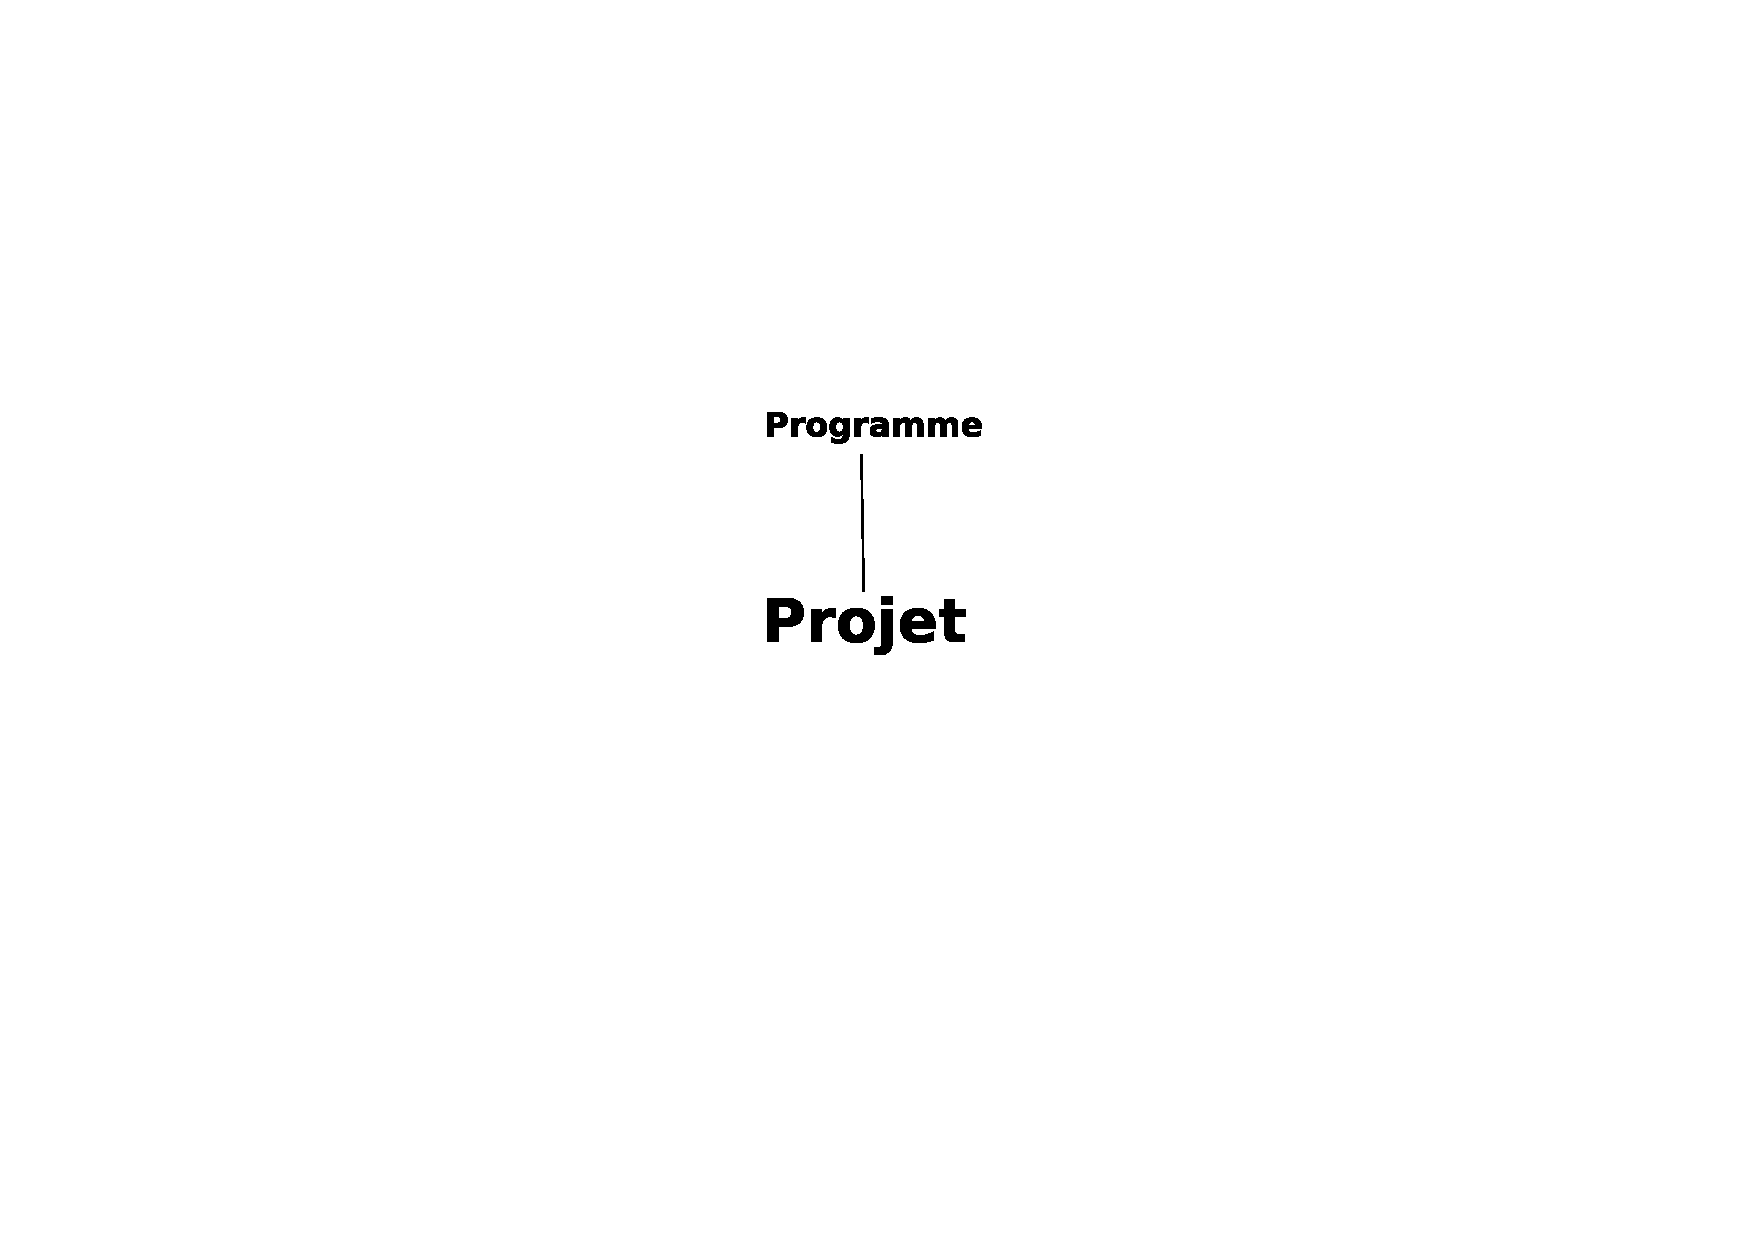
\includegraphics[height=200px]{brainstorming-2.pdf}}
      % Votre projet, c’est de concevoir un programme. Ah, c’est un peu plus
      % précis.
      \only<3>{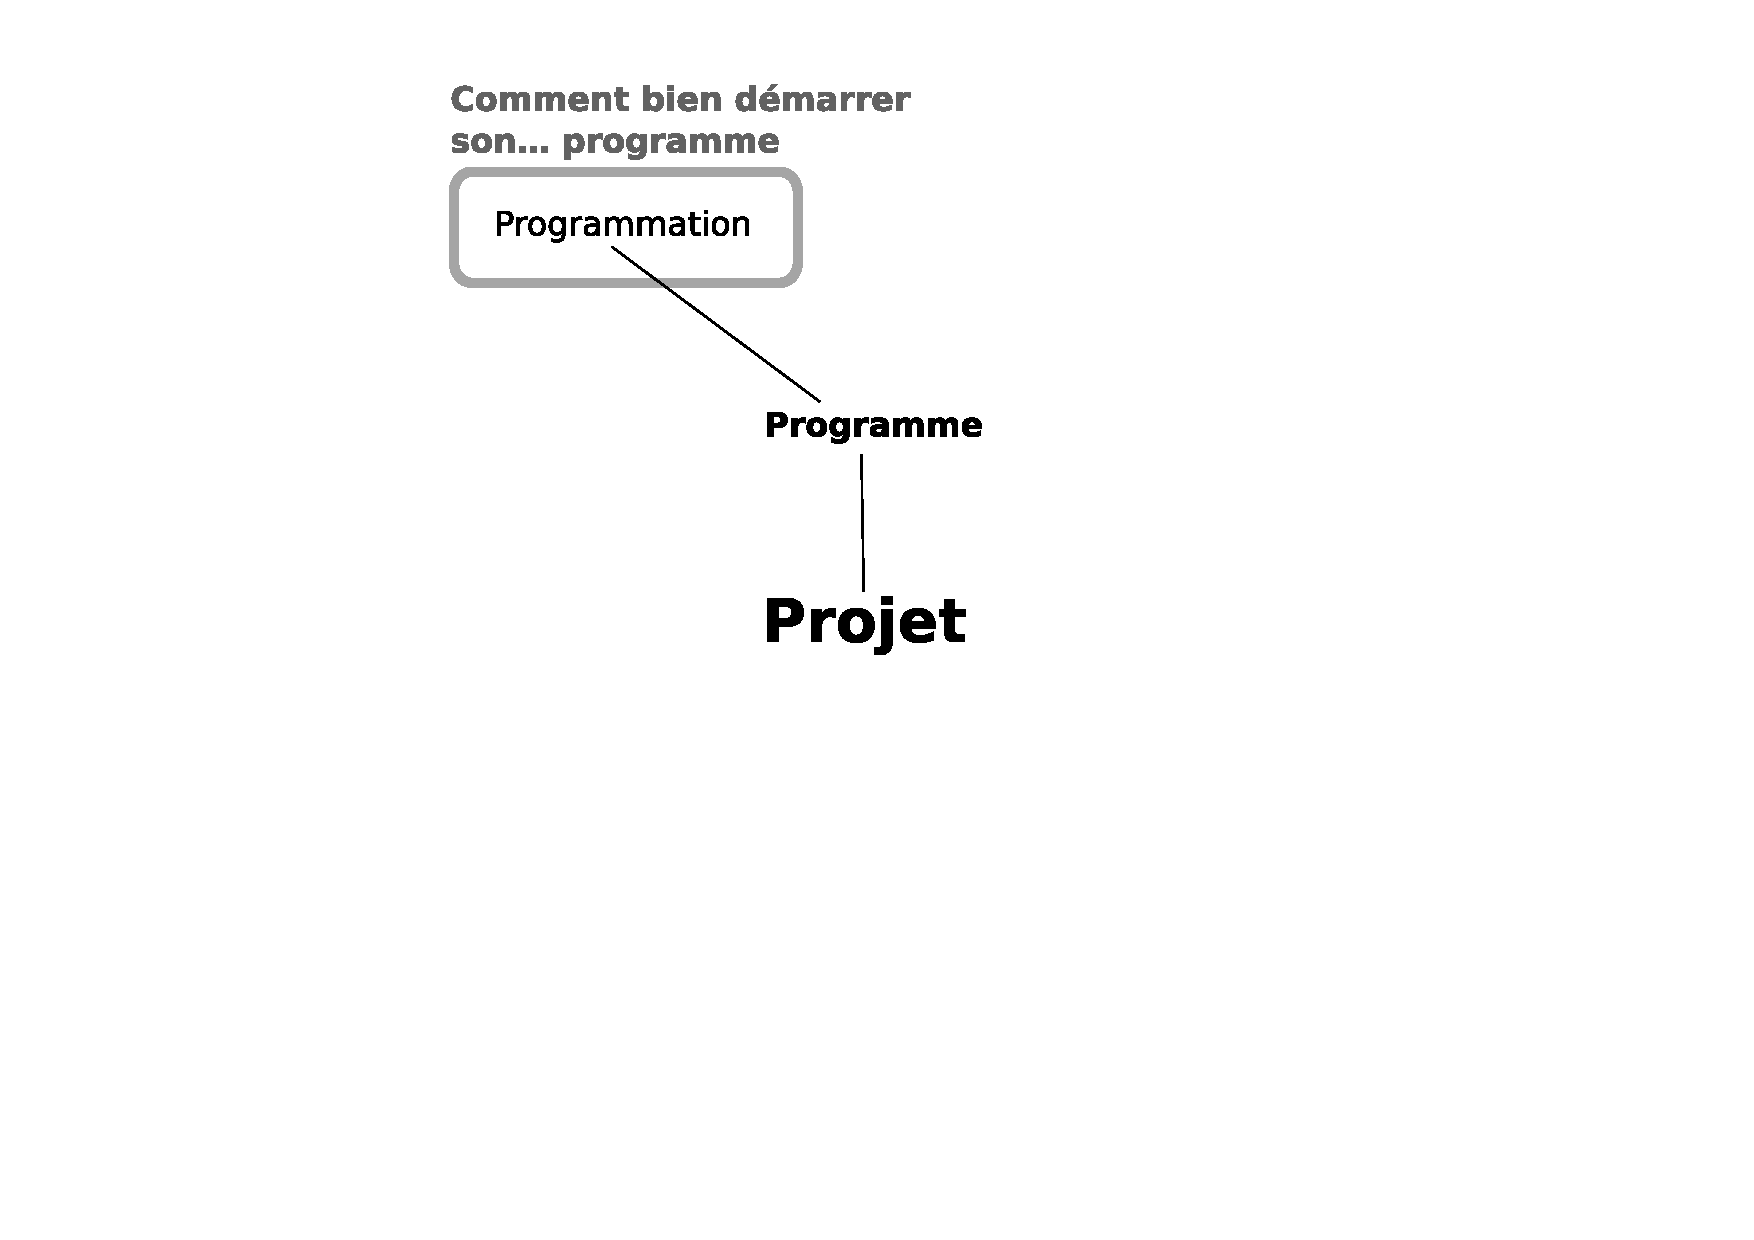
\includegraphics[height=200px]{brainstorming-3.pdf}}
      % Du coup, il va falloir que vous programmiez un peu. Logique. C’est le
      % premier volet de cette conférence : comment allez-vous vous y prendre ?
      \only<4>{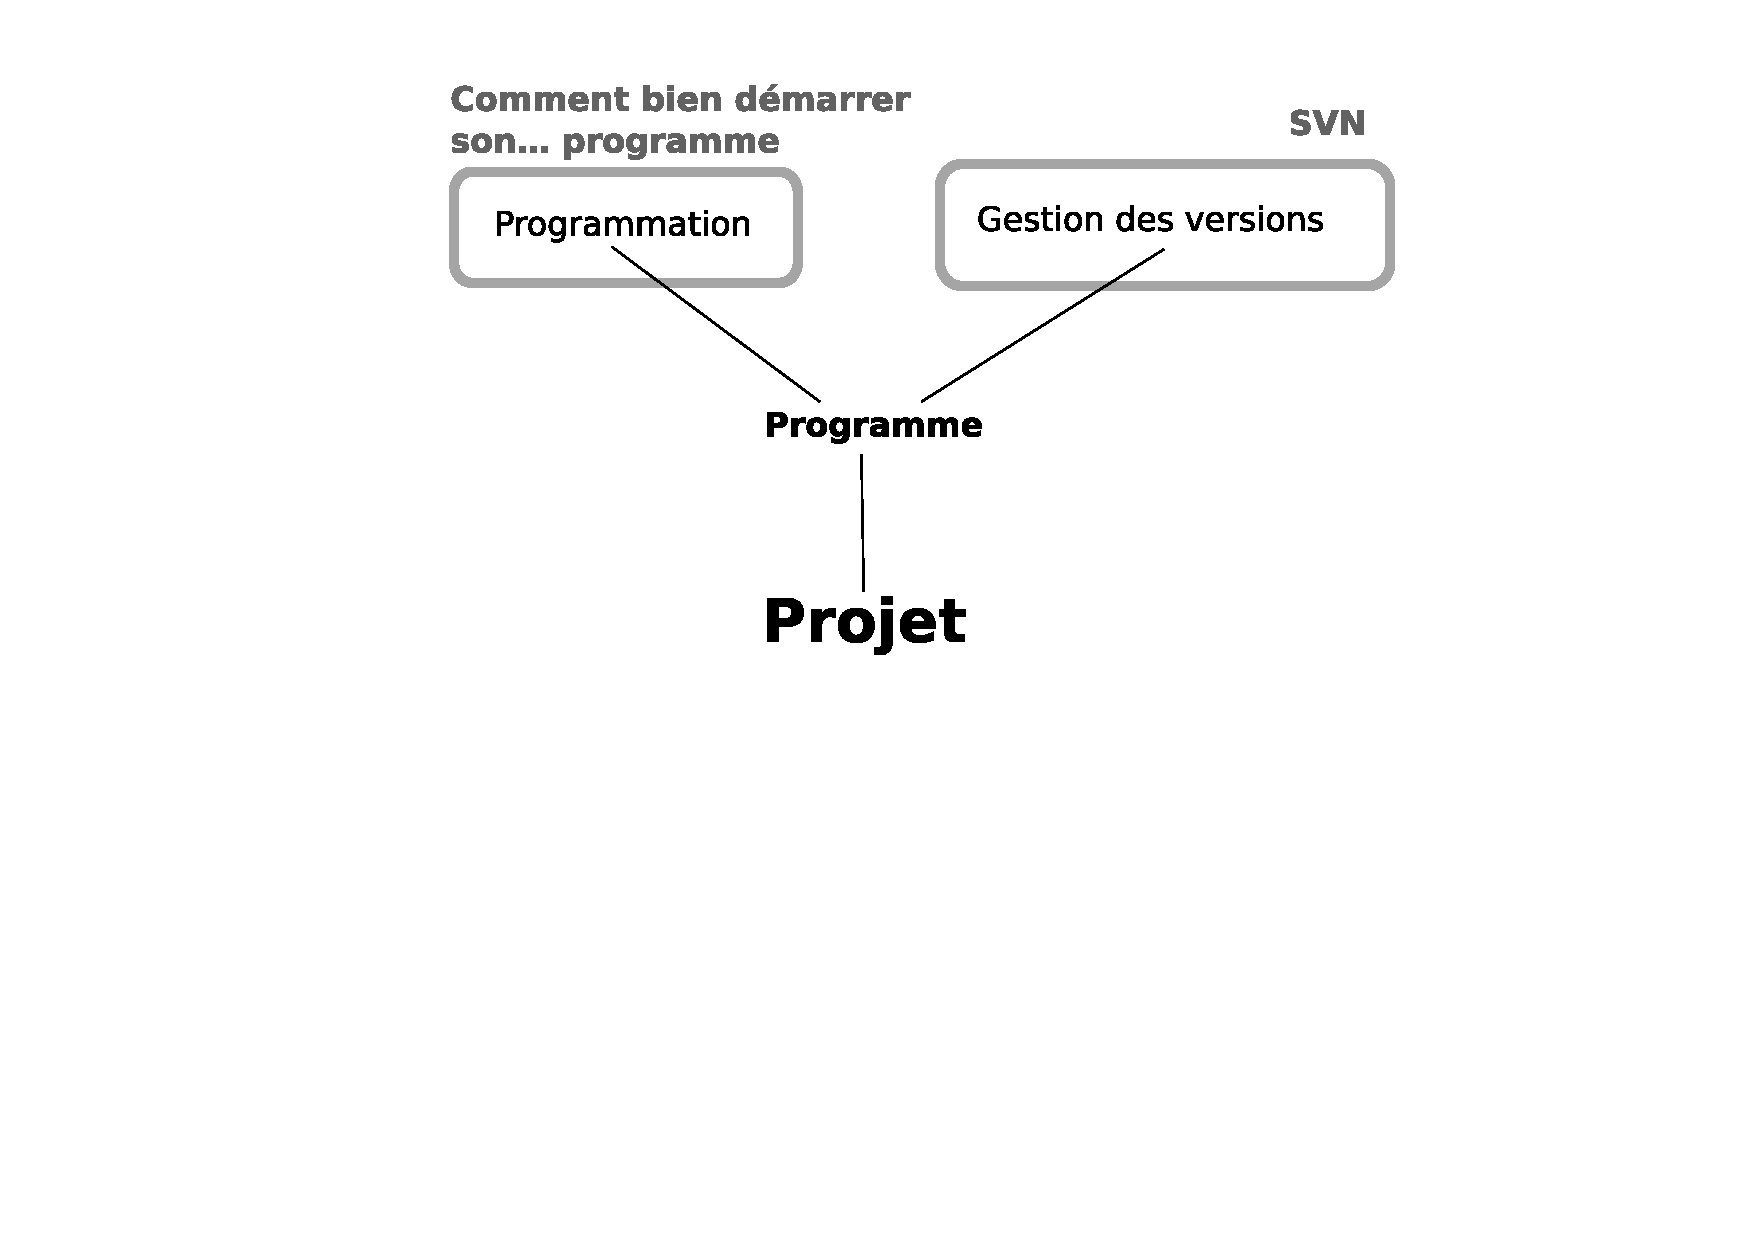
\includegraphics[height=200px]{brainstorming-4.pdf}}
      % Le code, c’est bien, mais… il faut maîtriser son évolution ! SVN, Git,
      % Mercucial et d’autres sont là pour vous faciliter la tâche. La deuxième
      % partie de cette conférence porte sur le principe et l’utilisation de SVN.
      \only<5>{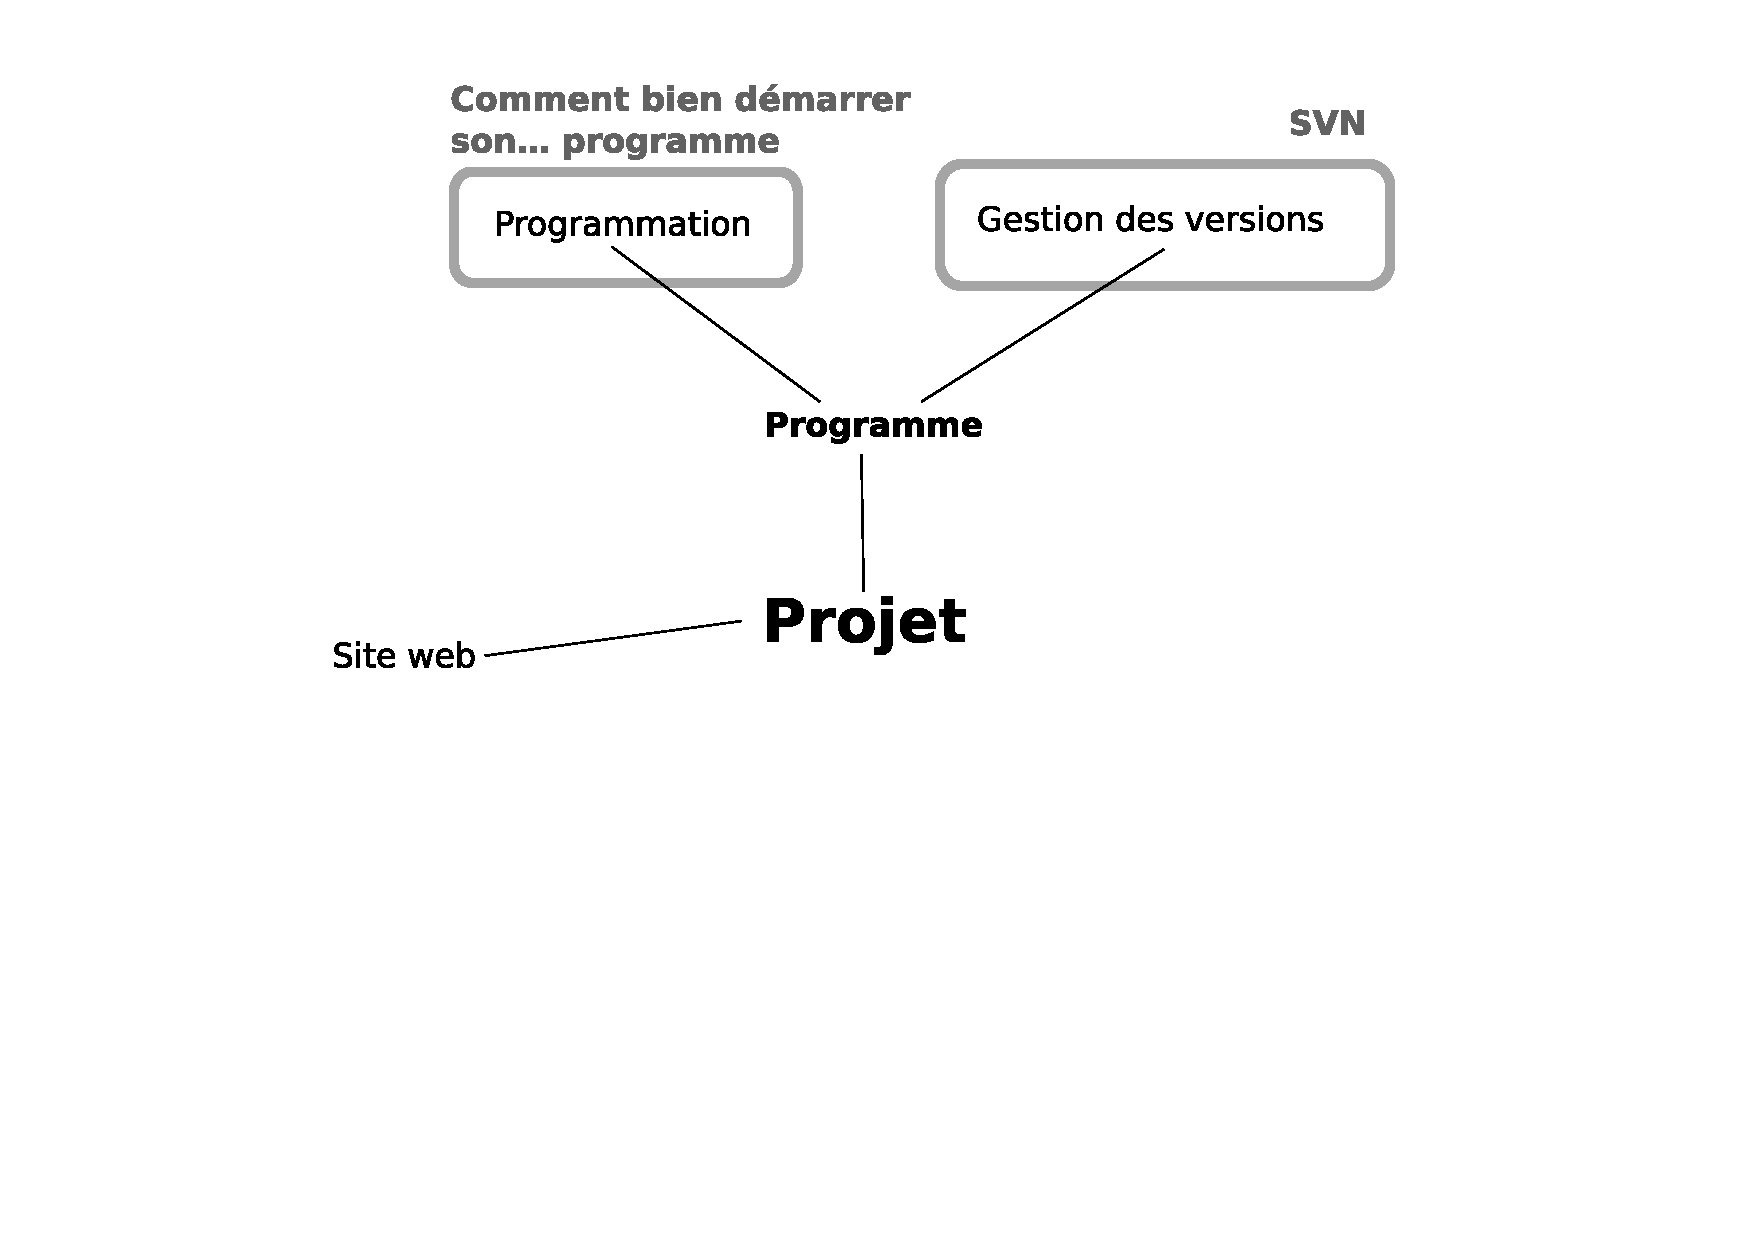
\includegraphics[height=200px]{brainstorming-5.pdf}}
      % Bon, le projet exige que vous concoctiez aussi un site web, une vitrine
      % de votre projet. Le site est assez important, comme toute la
      % communication autour de votre projet, mais ça reste simple et facile à
      % faire… Débrouillez-vous ! :-)
      \only<6>{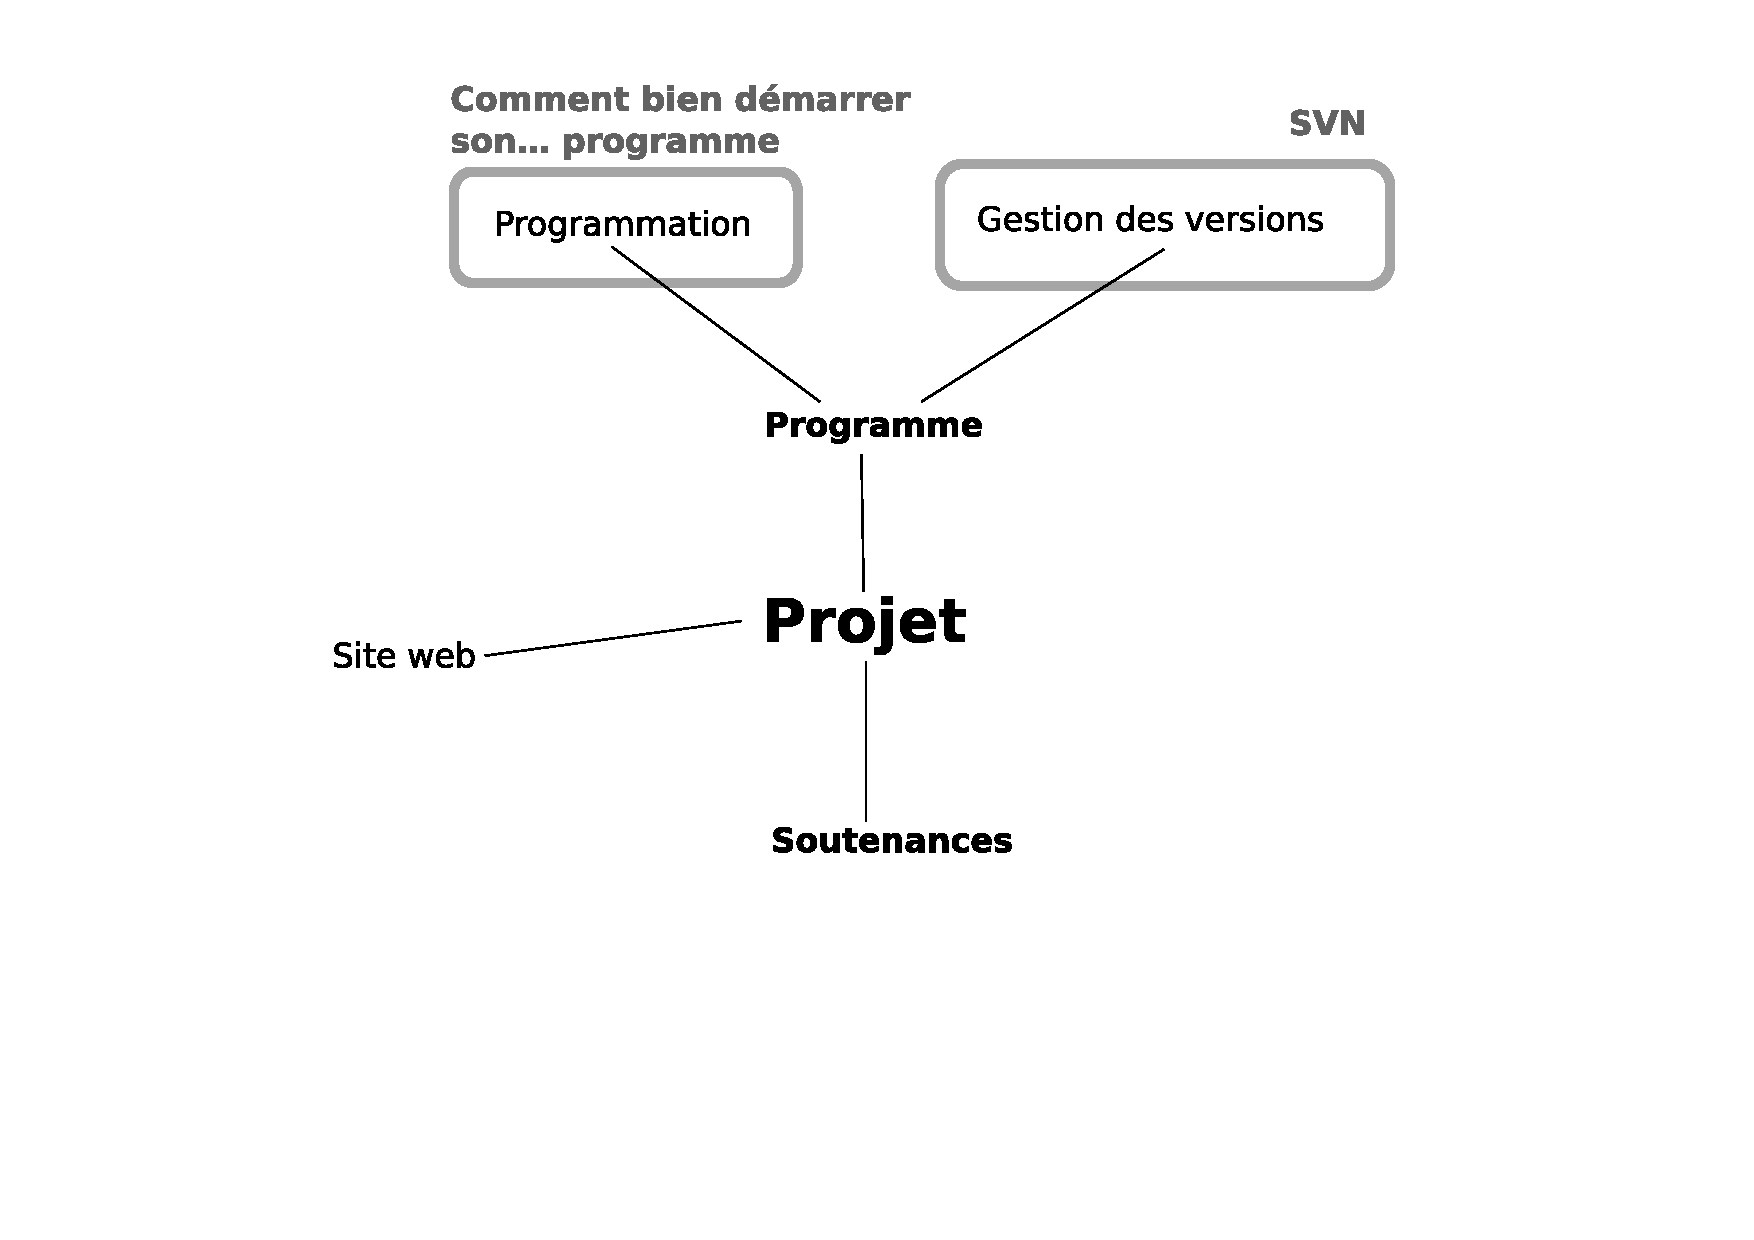
\includegraphics[height=200px]{brainstorming-6.pdf}}
      % Krisboul vous donne du travail et veut vous observer pour être certain
      % que vous bossez ! C’est pour cela que 4 soutenances sont prévues tout au
      % long de l’année.
      \only<7>{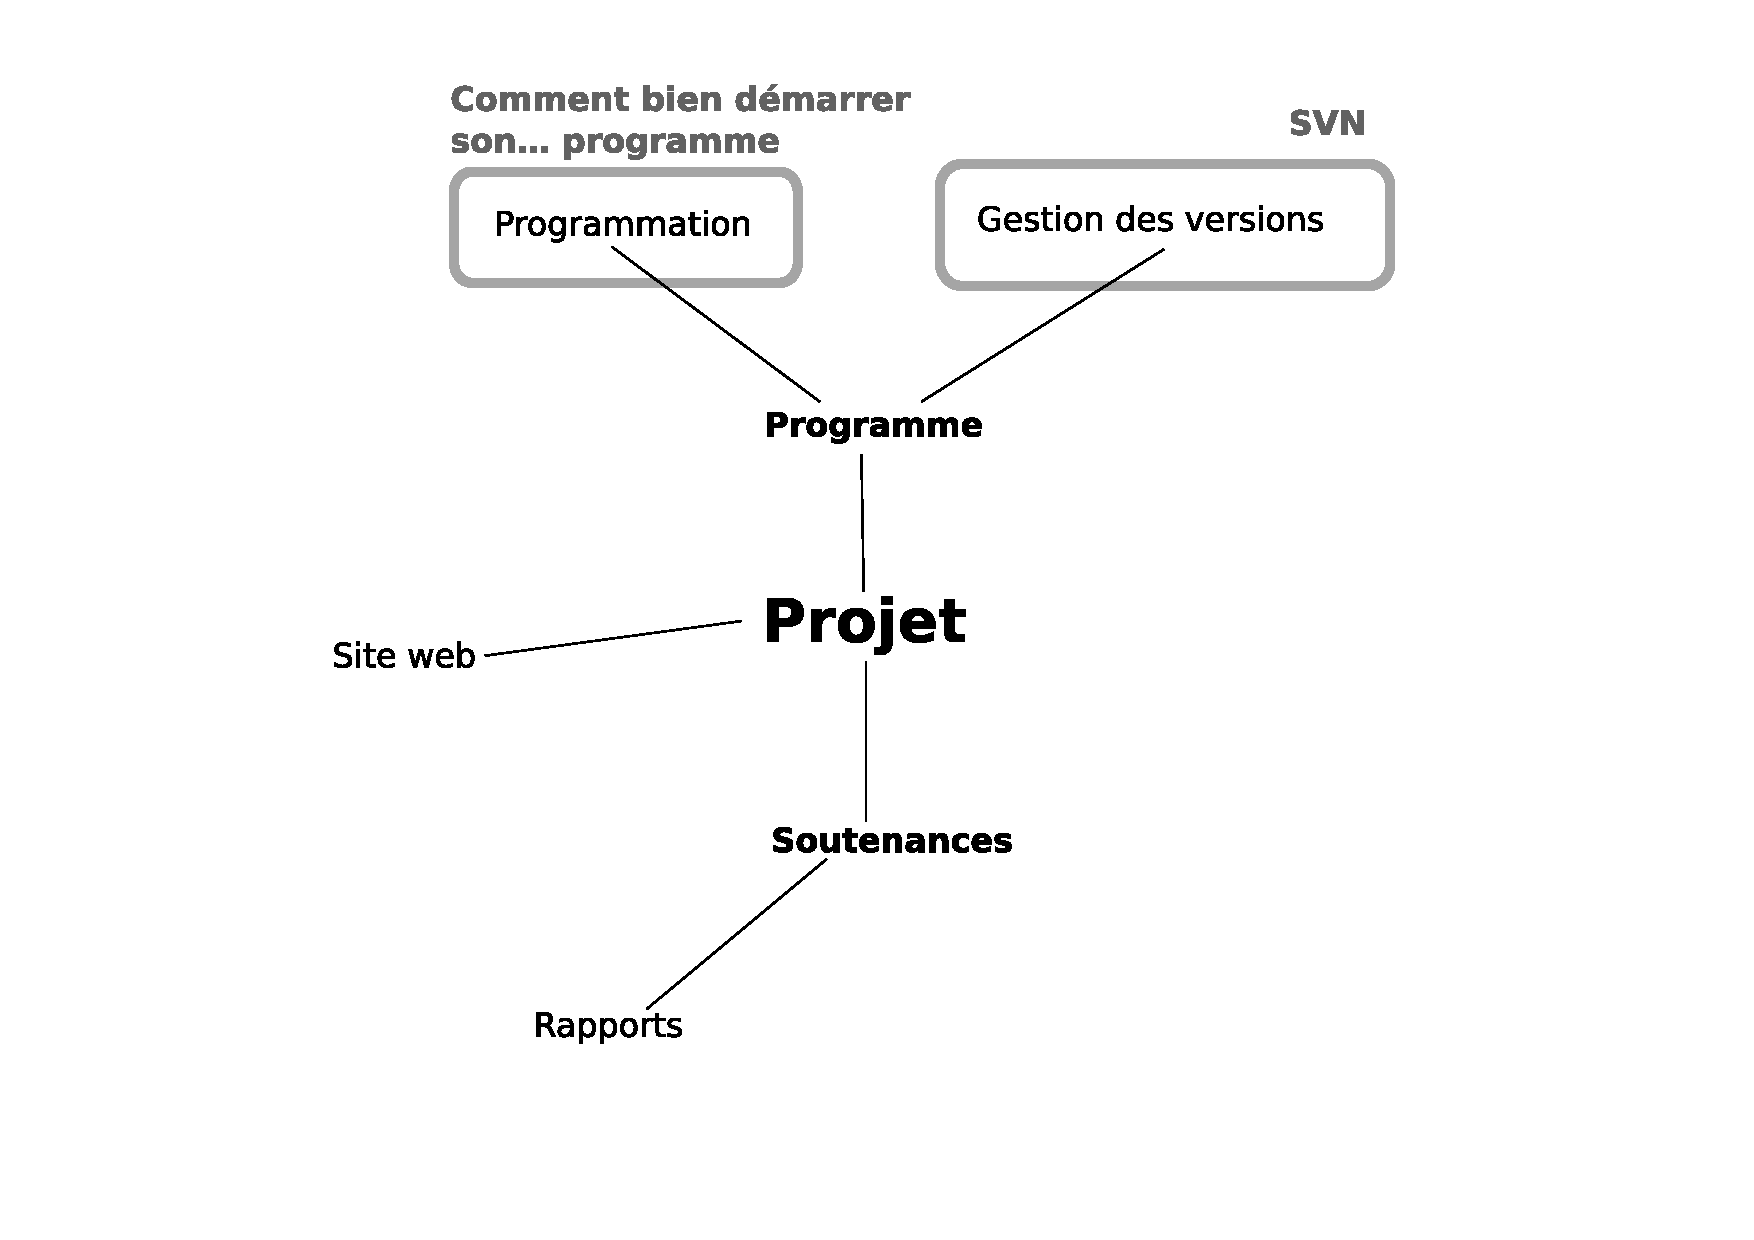
\includegraphics[height=200px]{brainstorming-7.pdf}}
      % À chaque soutenance, vous avez un rapport à fournir…
      \only<8>{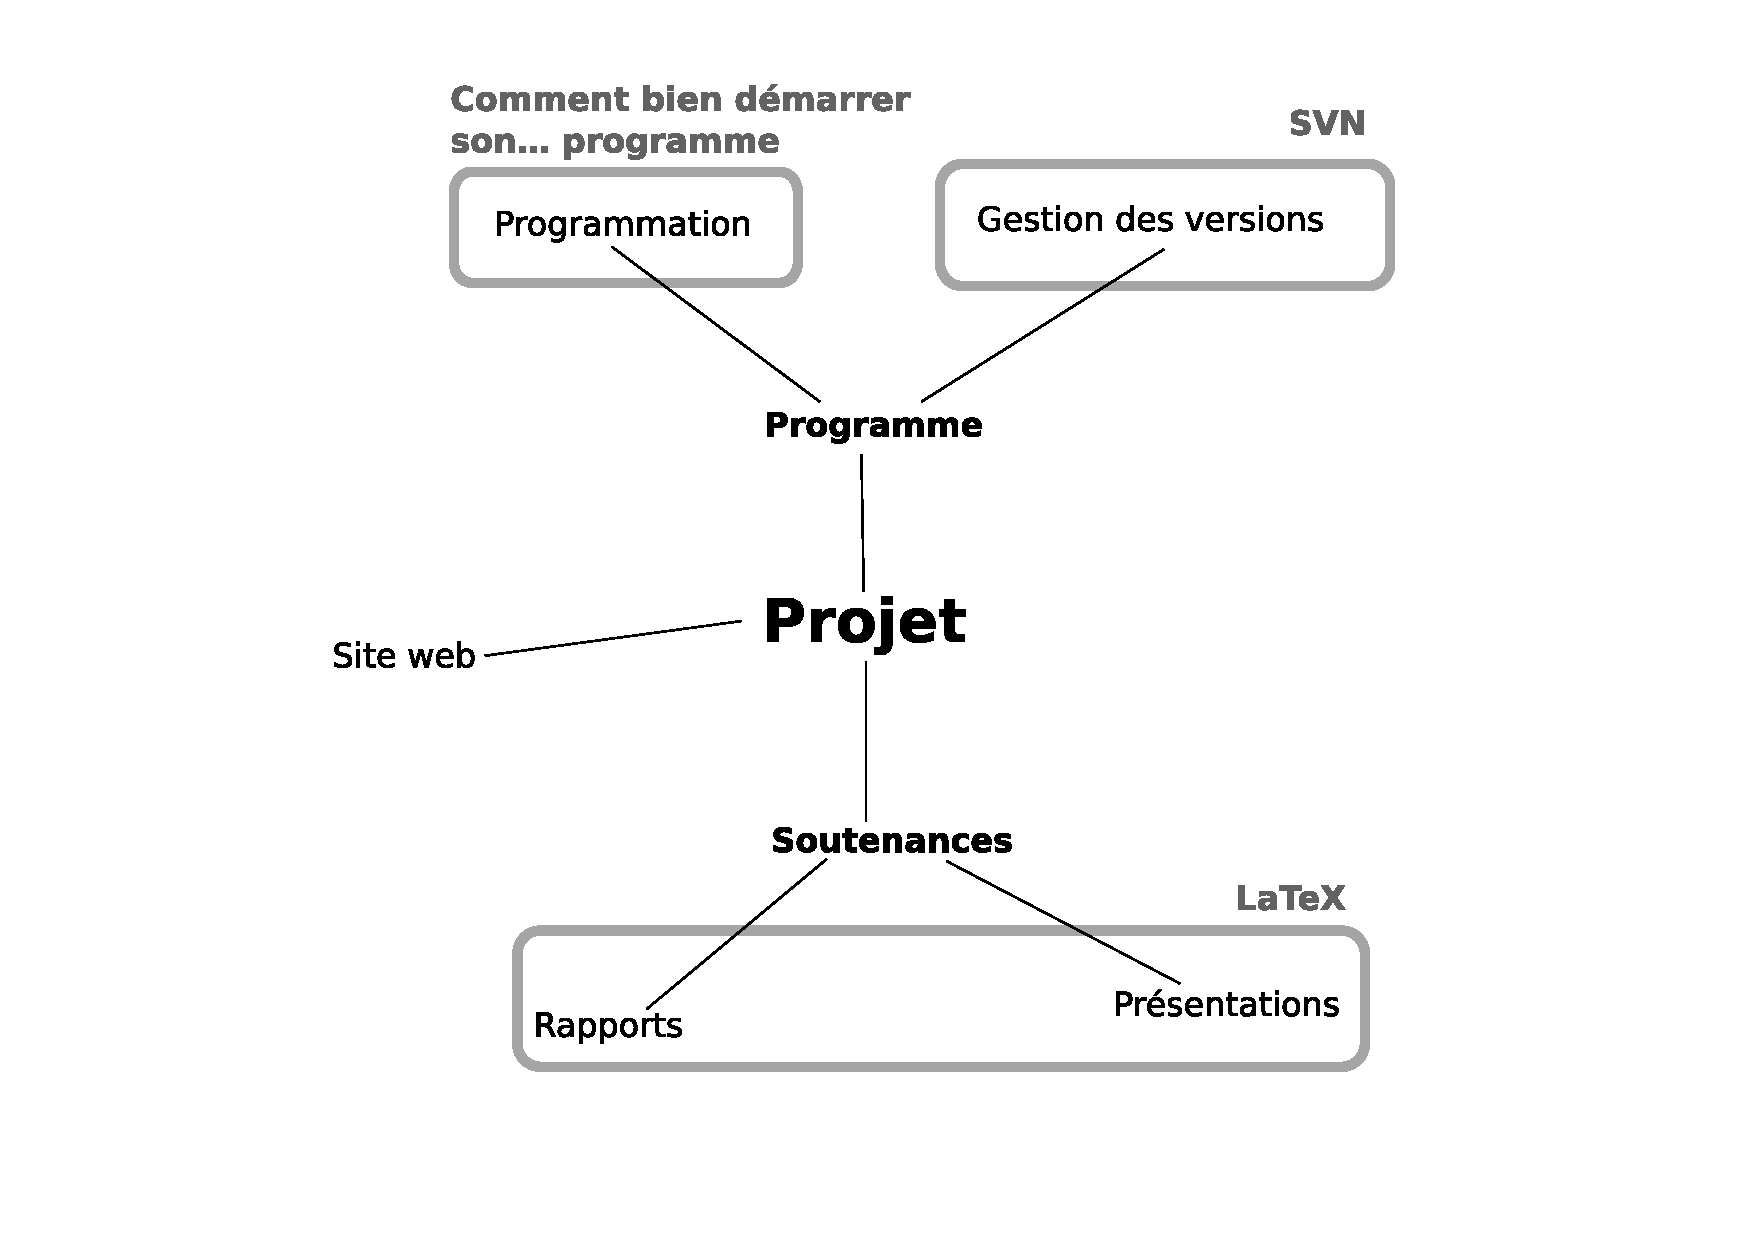
\includegraphics[height=200px]{brainstorming-8.pdf}}
      % … ainsi qu’une présentation à faire. Le contenu n’est pas l’objet de la
      % conférence (c’est dans le sujet, le reste n’est que quelques conseils
      % qu’on peut vous donner), en revanche nous vous conseillons d’utiliser
      % LaTeX pour mettre en forme vos rapports et vos diaporamas.
      \only<9>{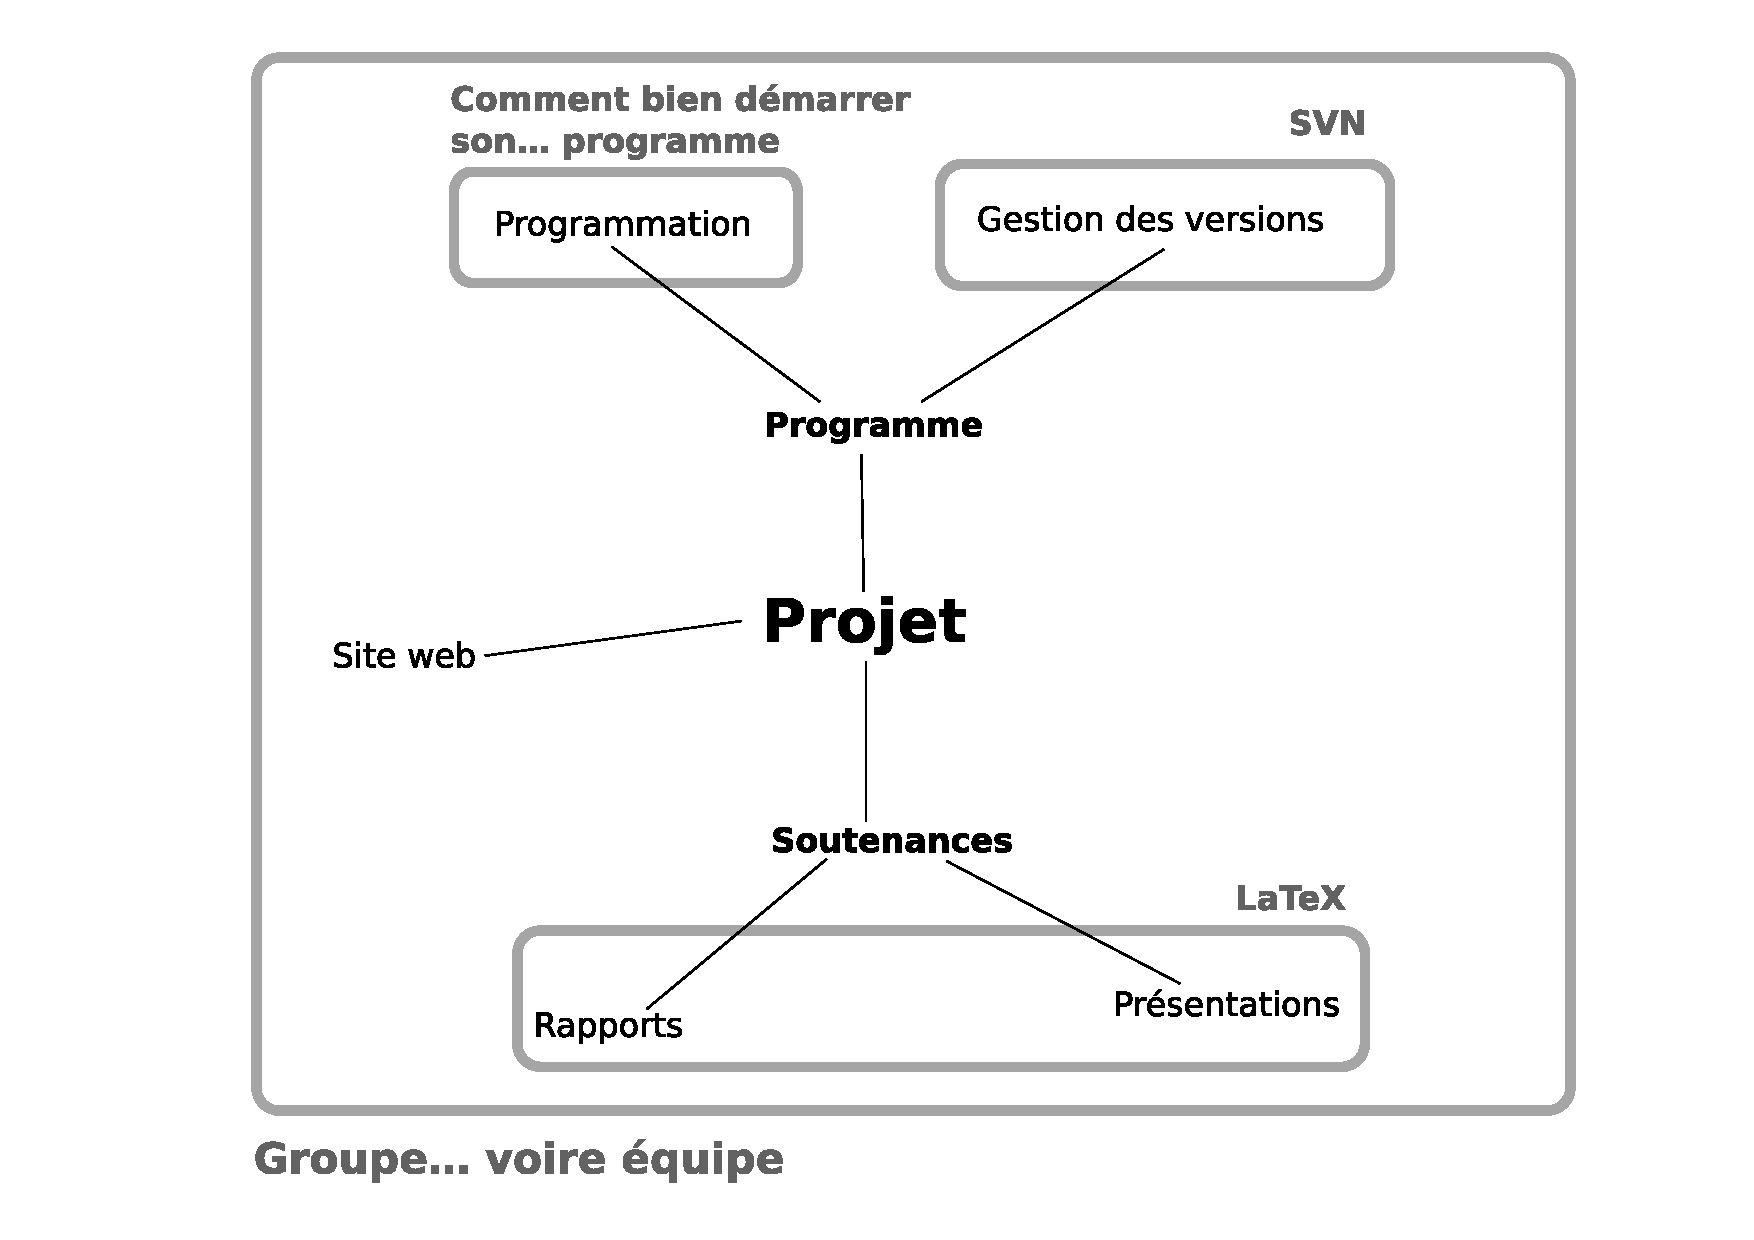
\includegraphics[height=200px]{brainstorming-9.pdf}}
      % Tout ce qui touche à votre projet est à faire en équipe. La gestion de
      % l’équipe est extrêmement importante ! … mais ce n’est pas ici qu’on va
      % vous expliquer comment vous y prendre.
      
    \end{overlayarea}
  \end{center}
\end{frame}


%%%
% Conférence « Comment bien démarrer son projet »
% Vendredi 13 novembre 2009
% Partie « Programmation » par Pierre-Marie de Rodat
%%%

\section{Programmation}

\subsection{Bien architecturer son projet}

\begin{frame}
    \begin{block}{Pourquoi ?}
        \begin{itemize}
            \item Rend plus aisé l'ajout de fonctionnalités
            \item Facilite la recherche et la correction de bugs
            \item Facilite la compréhension du code dans l'équipe
            \item Rend possible le travail en groupe
        \end{itemize}
    \end{block}
\end{frame}


\begin{frame}
    \begin{block}{Comment ?}
        \begin{itemize}
            \item Prendre du recul sur le projet et abstraire les problèmes
            \item Réfléchir avant de coder
            \item Refactoriser en permanence
        \end{itemize}
    \end{block}
\end{frame}

\begin{frame}
  Dressez un descriptif rapide de votre projet.
  \begin{center}
    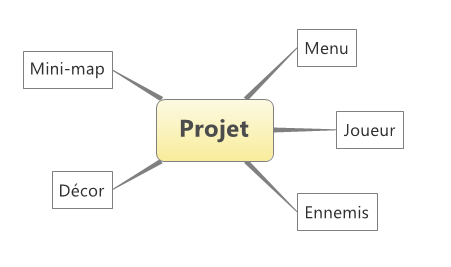
\includegraphics[scale=0.6]{images/project_overview.png}
  \end{center}
\end{frame}


%%%
% Conférence « Comment bien démarrer son projet »
% Vendredi 03 décembre 2010
%%%

\section{Subversion}

\subsection{Généralités}
\begin{frame}{Pourquoi versionner~?}
  \begin{alertblock}{Concrètement}
    SVN vous permet de~:
    \begin{itemize}
      \item gérer votre code source,
      \item conserver une trace toutes les modifications,

      \item revenir en arrière,
      \item travailler à plusieurs en partageant le code intelligement.
    \end{itemize}
  \end{alertblock}
  \begin{center}
    
\includegraphics[scale=3]{images/logo_svn}
  \end{center}
\end{frame}

\subsection{Utilisation typique}

\begin{frame}
  \begin{center}
    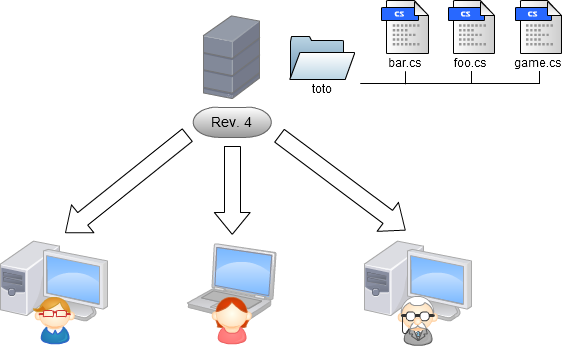
\includegraphics[scale=0.52]{images/1-CheckOut.png}
  \end{center}
\end{frame}

\begin{frame}
  \begin{center}
    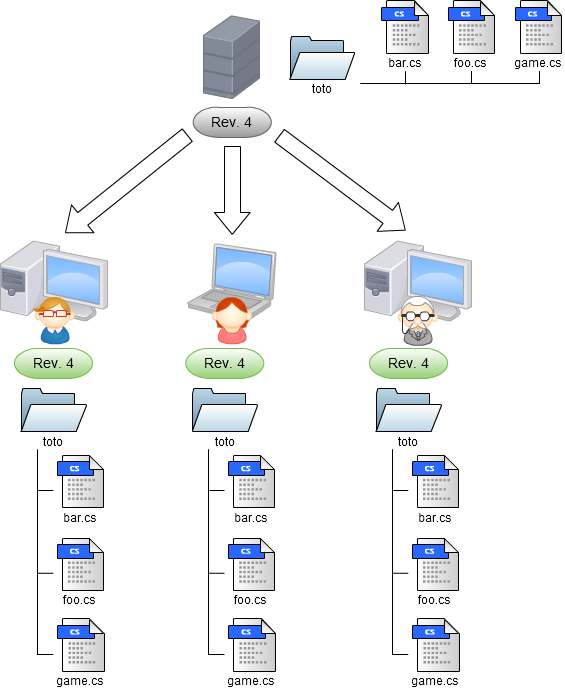
\includegraphics[scale=0.3]{images/2-CheckOut.png}
  \end{center}
\end{frame}

\begin{frame}
  \begin{center}
    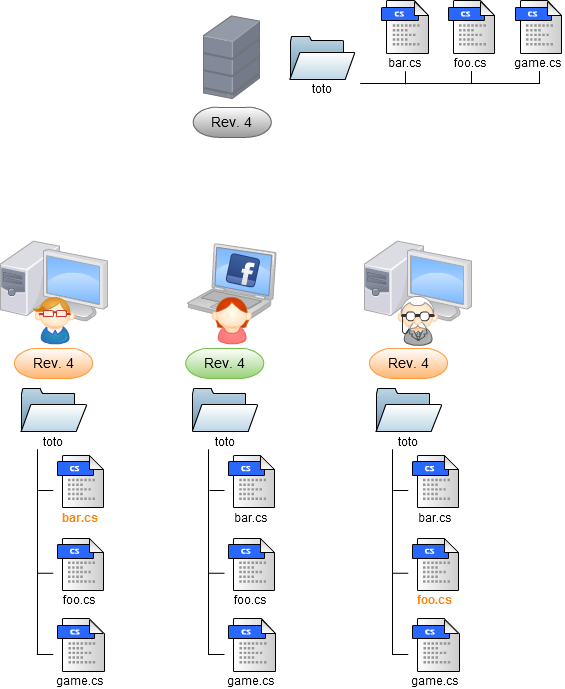
\includegraphics[scale=0.3]{images/3-Work.png}
  \end{center}
\end{frame}

\begin{frame}
  \begin{center}
    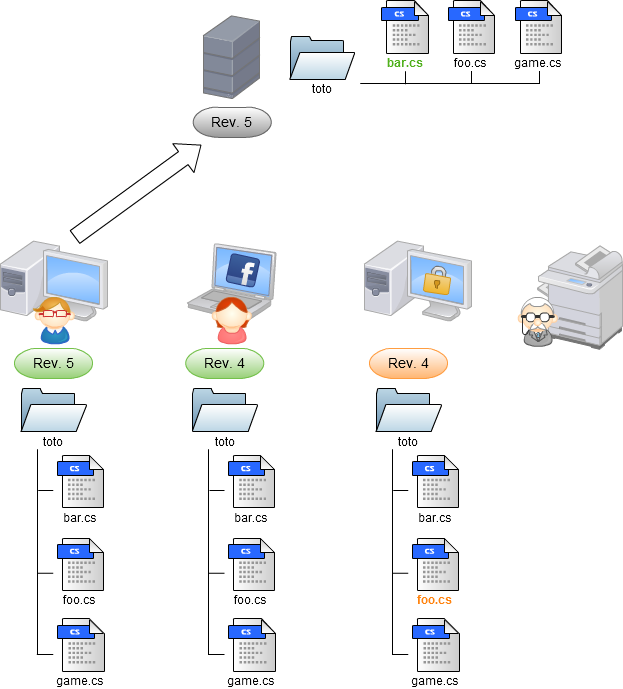
\includegraphics[scale=0.3]{images/4-Commit1.png}
  \end{center}
\end{frame}

\begin{frame}
  \begin{center}
    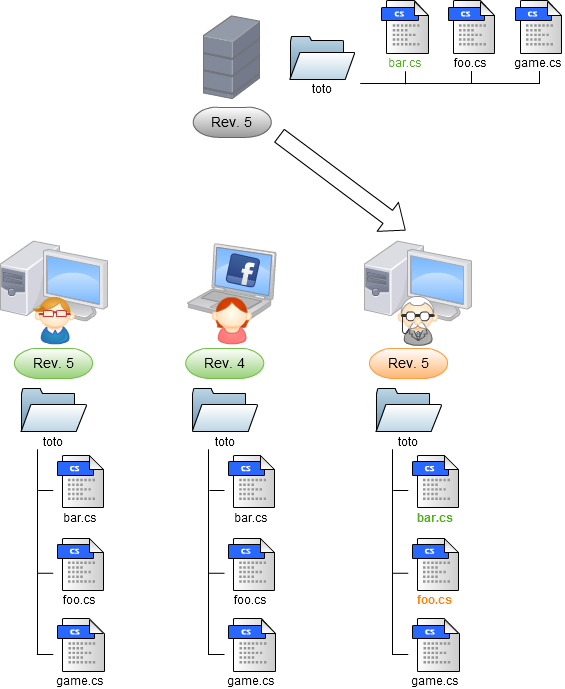
\includegraphics[scale=0.3]{images/5-Update.png}
  \end{center}
\end{frame}

\begin{frame}
  \begin{center}
    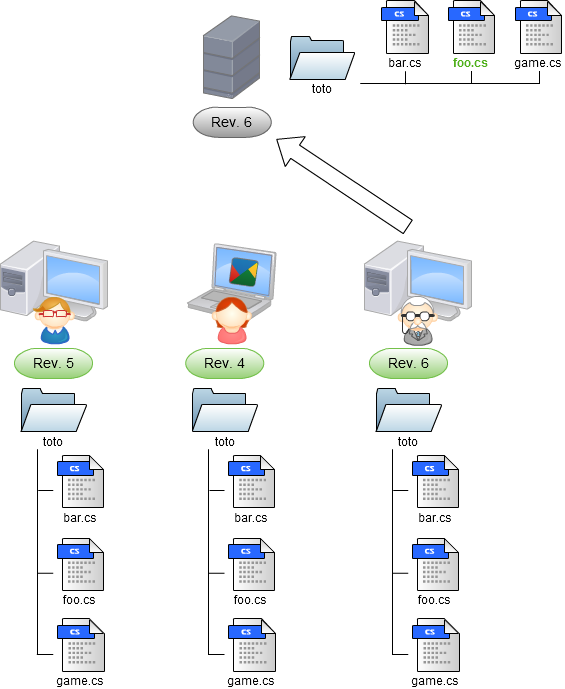
\includegraphics[scale=0.3]{images/6-Commit2.png}
  \end{center}
\end{frame}

\begin{frame}
  \begin{center}
    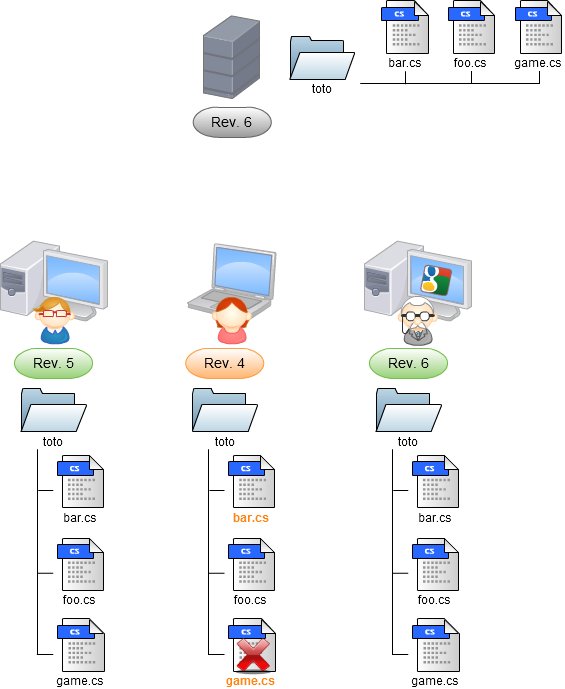
\includegraphics[scale=0.3]{images/7-Work.png}
  \end{center}
\end{frame}

\begin{frame}
  \begin{center}
    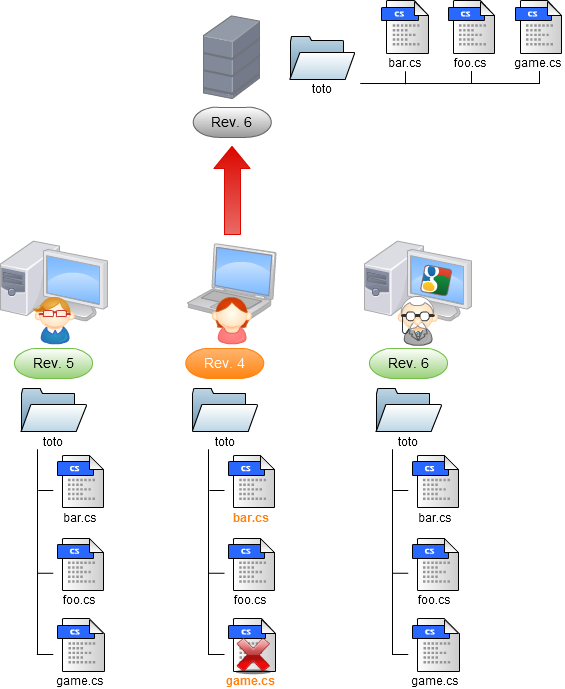
\includegraphics[scale=0.3]{images/8-Commit3.png}
  \end{center}
\end{frame}

\begin{frame}
  \begin{center}
    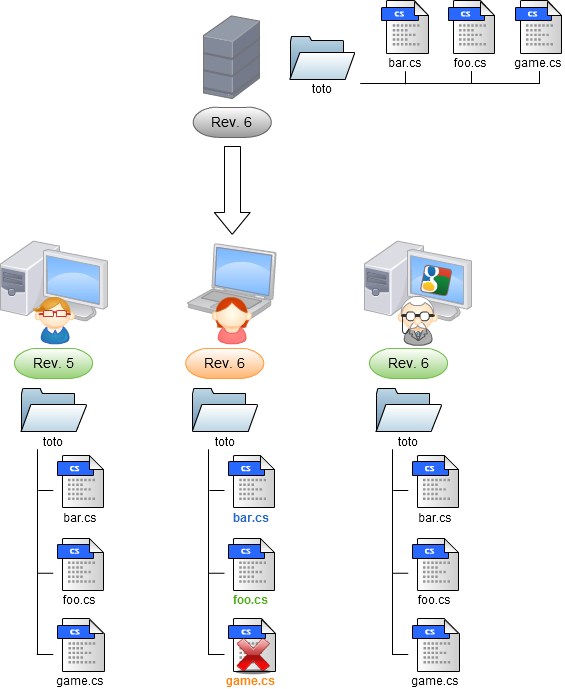
\includegraphics[scale=0.3]{images/9-Update_merge.png}
  \end{center}
\end{frame}

\begin{frame}
  \begin{center}
    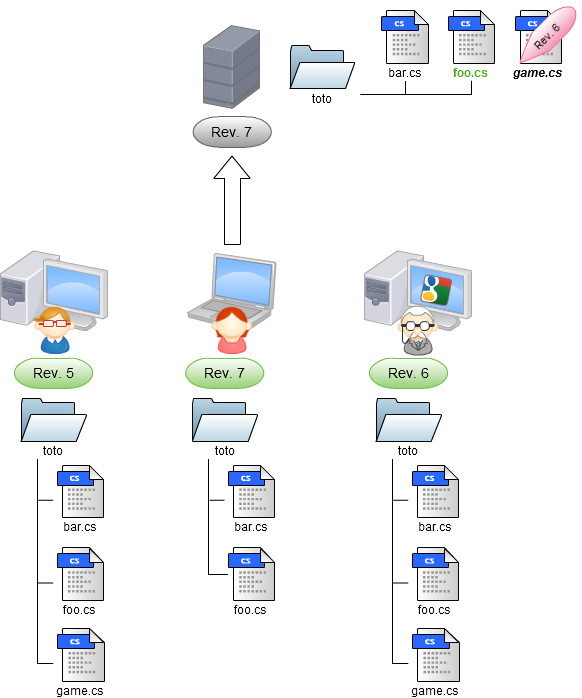
\includegraphics[scale=0.3]{images/10-Commit4.png}
  \end{center}
\end{frame}

\begin{frame}
  \begin{center}
    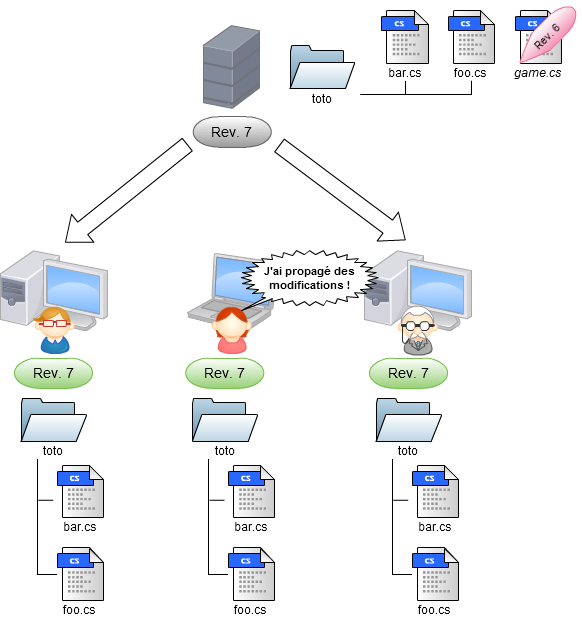
\includegraphics[scale=0.3]{images/11-Update.png}
  \end{center}
\end{frame}

\begin{frame}
  \begin{center}
    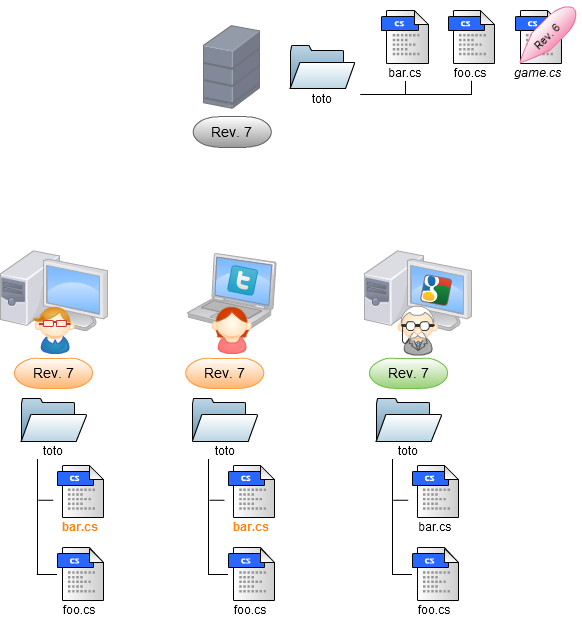
\includegraphics[scale=0.3]{images/12-Work.png}
  \end{center}
\end{frame}

\begin{frame}
  \begin{center}
    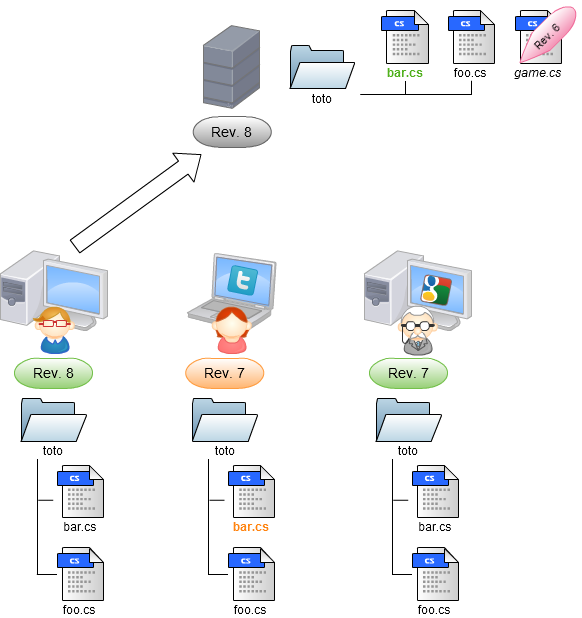
\includegraphics[scale=0.3]{images/13-Commit4.png}
  \end{center}
\end{frame}

\begin{frame}
  \begin{center}
    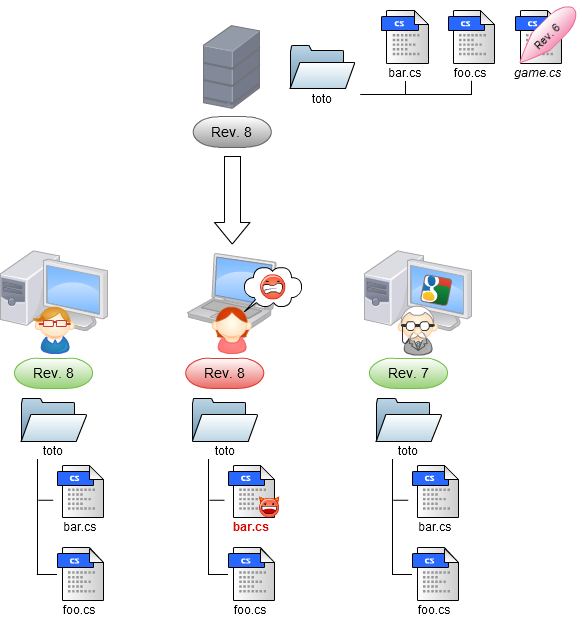
\includegraphics[scale=0.3]{images/14-Conflict.png}
  \end{center}
\end{frame}

\begin{frame}
  \begin{center}
    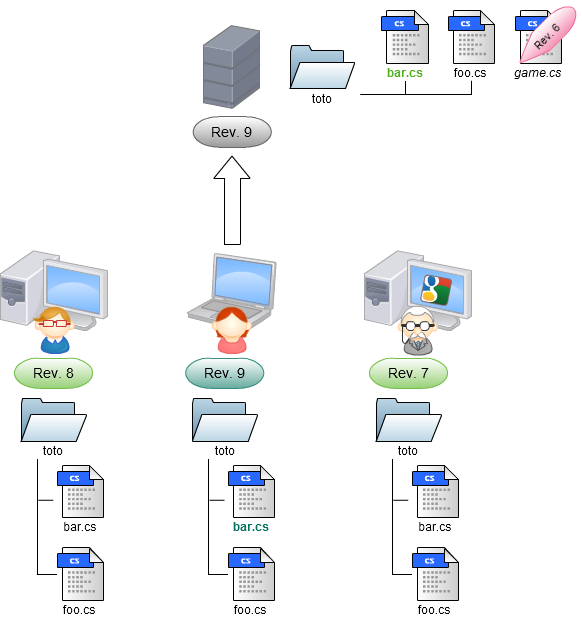
\includegraphics[scale=0.3]{images/15-Resolved.png}
  \end{center}
\end{frame}

\begin{frame}
  \begin{center}
    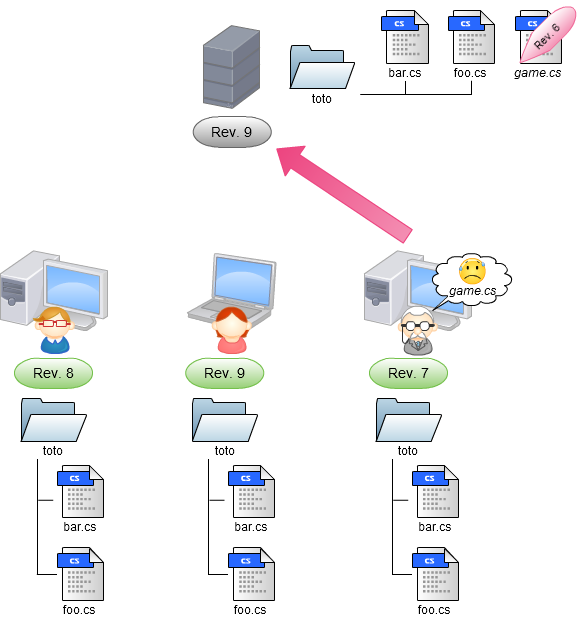
\includegraphics[scale=0.3]{images/16-Back1.png}
  \end{center}
\end{frame}


\subsection{Commandes usuelles}

\begin{frame}{Subversion survival package}
  \begin{block}{Checkout -- co}
    Récupération du contenu d'un dépôt (désigné par une URL) à une version donnée.
  \end{block}
  \begin{block}{Update -- up}
    Mise à jour du contenu d'un dossier/fichier sous versionnement par rapport à la référence.
  \end{block}
  \begin{block}{Commit -- ci}
    Enregistrement des modifications effectuées sur le serveur.
  \end{block}
  \begin{block}{Add}
    Activer le versionnement sur un dossier/fichier.
  \end{block}
\end{frame}

\subsection{Environnement de travail}
\begin{frame}
  \begin{center}
    
\includegraphics[scale=0.35]{images/logo_tortoise}
  \end{center}
  \begin{alertblock}{TortoiseSVN}
    \begin{itemize}
    \item S'intégre parfaitement à Windows,
    \item Ajout d'action sur les fichiers et dossiers (clic droit),
      \item Modification visuelle pour les dossiers et fichiers sous versionnement.
      \end{itemize}
    \end{alertblock}
\end{frame}

\begin{frame}
  \begin{figure}
    \begin{center}
      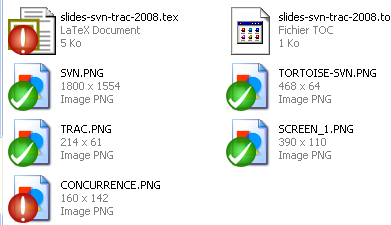
\includegraphics[scale=0.7]{images/dirView}
    \end{center}
  \end{figure}
\end{frame}
\begin{frame}
  \begin{figure}
    \begin{center}
      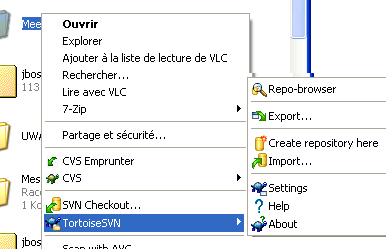
\includegraphics[scale=0.7]{images/actions}
    \end{center}
  \end{figure}
\end{frame}

\subsection{Bonnes pratiques}
\begin{frame}
  \begin{alertblock}{Update}
    Effectuer des updates régulièrement.
  \end{alertblock}
  \begin{alertblock}{Commit}
    Commiter \textbf{régulièrement} du code qui \textbf{compile}.
  \end{alertblock}
  \begin{alertblock}{Add}
    Ne pas mettre sous versionnement~:
    \begin{itemize}
    \item Les fichiers compilés par votre code (.exe, .o, .out, \ldots),
    \item Les fichiers propres à votre environnement de travail,
    \item Les fichiers systèmes (Thumbs.db, \ldots),
    \item Des fichiers inutiles (SVN n'est pas un système de partage de fichiers).
    \end{itemize}
  \end{alertblock}
\end{frame}

\subsection{Où trouver un dépôt~?}
\begin{frame}
  \begin{exampleblock}{Les dépôts gratuits}
    \begin{itemize}
    \item GoogleCode
    \item SourceForge
    \item Assembla
    \item svn.pc-show.com
    \end{itemize}
  \end{exampleblock}
\end{frame}


%%%
% Conférence « Comment bien démarrer son projet »
% Vendredi 03 décembre 2010
%%%

\section{Soutenances}

\subsection{Généralités}
\begin{frame}
  \begin{block}{Points clés}
    \begin{itemize}
    \item Capter l'attention de \emph{Krisboul},
    \item 13 à 15 minutes,
    \item être fier de son jeu,
    \item être en avance sur le planing.
    \end{itemize}
  \end{block}
\end{frame}

\begin{frame}
  \begin{block}{Le site internet}
    \begin{itemize}
    \item La vitrine du projet,
    \item noté dès la deuxième soutenance,
    \item être simple, beau, avec du contenu \textbf{à jour}.
    \end{itemize}
  \end{block}
\end{frame}

\begin{frame}
  \begin{block}{Les rapports}
    \begin{itemize}
    \item \LaTeX,
    \item environ 20 pages,
    \item images, captures, dessins, à donf,
    \item s'inspirer des promos précédentes.
    \end{itemize}
  \end{block}
\end{frame}

\begin{frame}
  Au boulot~!
\end{frame}

\end{document}
